\section*{Anexo G – Análisis avanzado por fuente de datos}
\label{anexo:analisis_avanzado}
\addcontentsline{toc}{section}{Anexo G – Análisis avanzado por fuente de datos}

Este anexo contiene las gráficas avanzadas complementarias para el análisis exhaustivo realizado sobre los mejores modelos entrenados con cada fuente de datos (sourceId 1, 2 y 5). Estas gráficas permiten identificar visualmente patrones específicos, errores sistemáticos, posibles sesgos y áreas potenciales de mejora para futuros desarrollos del modelo.

\subsection*{SourceId 1}

\begin{figure}[H]
	\centering
	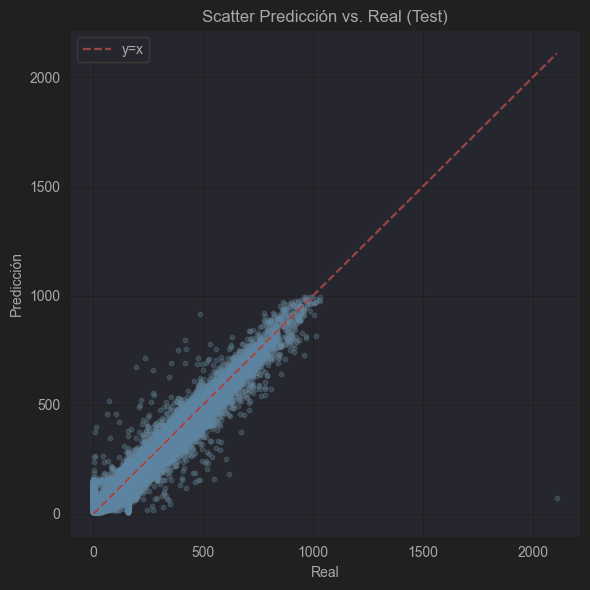
\includegraphics[width=0.75\linewidth]{includes/cap5/graphs/advanced/sid1_scatter_predicted_vs_actual.png}
	\caption{Gráfico de dispersión (predicción vs. valores reales) para SourceId 1.}
	\label{fig:sid1_scatter}
\end{figure}

\begin{figure}[H]
	\centering
	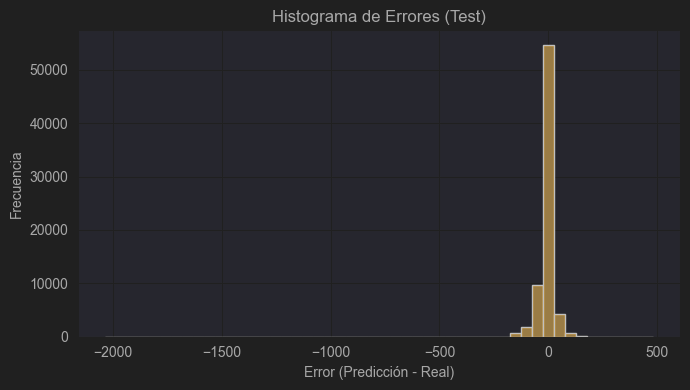
\includegraphics[width=0.75\linewidth]{includes/cap5/graphs/advanced/sid1_error_histogram_predicted_vs_actual.png}
	\caption{Histograma del error absoluto (residual) para SourceId 1.}
	\label{fig:sid1_histograma_error}
\end{figure}

\begin{figure}[H]
	\centering
	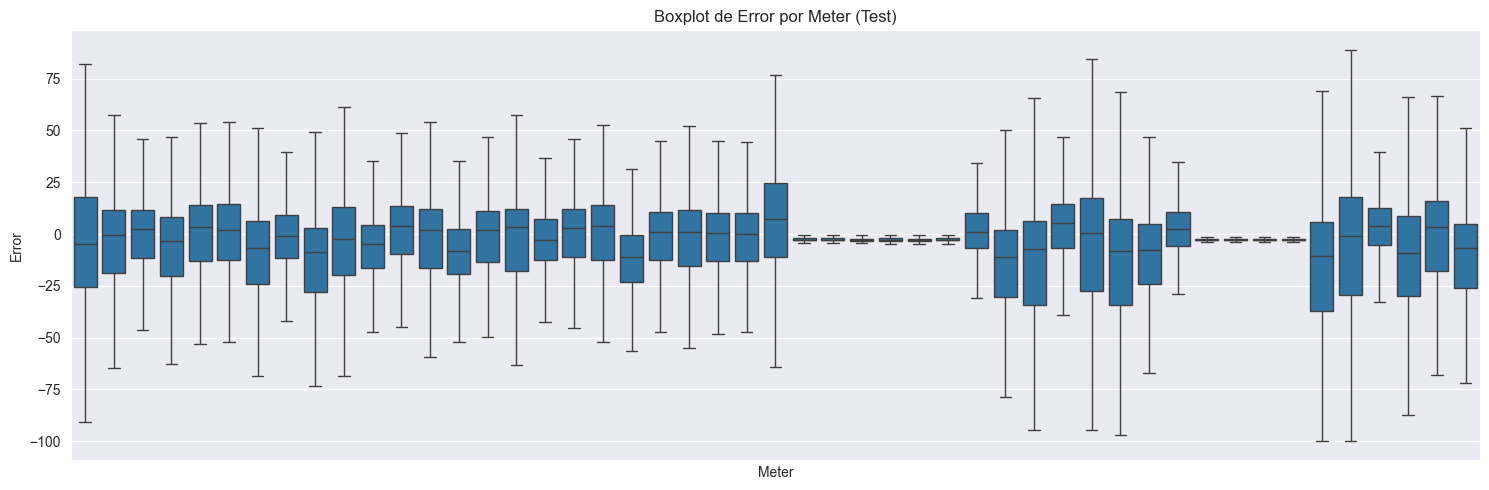
\includegraphics[width=0.75\linewidth]{includes/cap5/graphs/advanced/sid1_all_meters_error_boxplot.png}
	\caption{Boxplot del error absoluto por sensor para todos los sensores del SourceId 1.}
	\label{fig:sid1_boxplot_all}
\end{figure}

\begin{figure}[H]
	\centering
	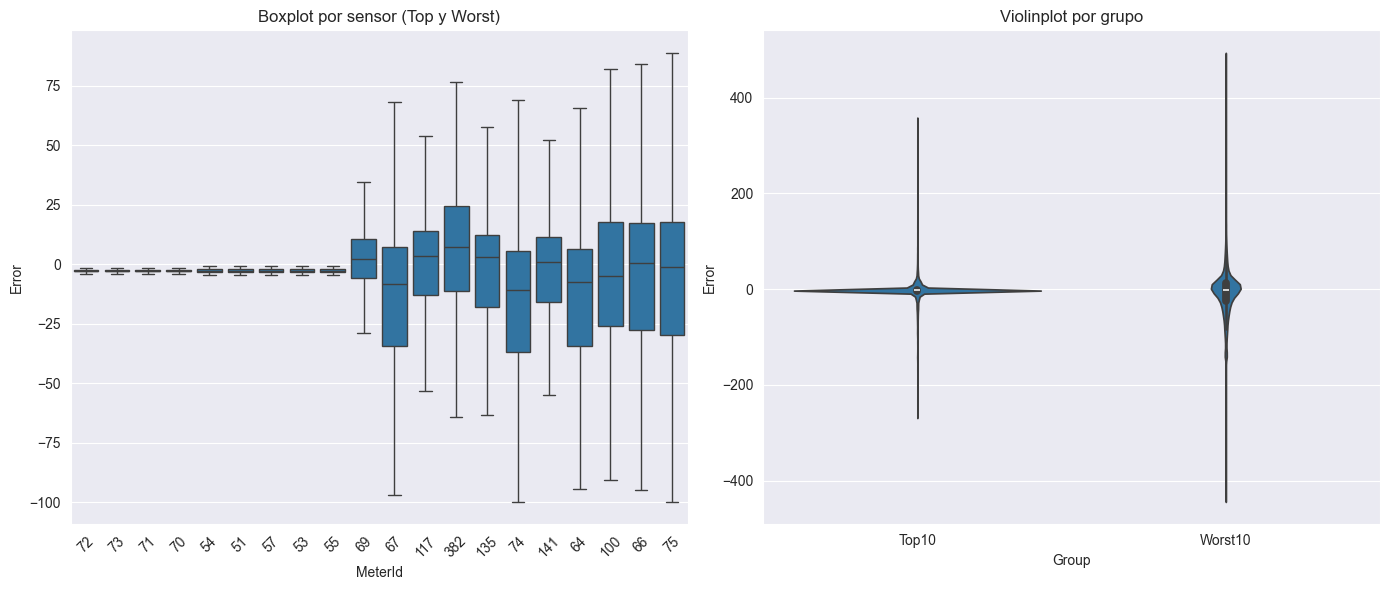
\includegraphics[width=0.75\linewidth]{includes/cap5/graphs/advanced/sid1_10best_10worst_meter_boxplot_violinplot.png}
	\caption{Boxplot y Violinplot de errores para los 10 mejores y los 10 peores sensores del SourceId 1.}
	\label{fig:sid1_violinplot_best_worst}
\end{figure}

\begin{figure}[H]
	\centering
	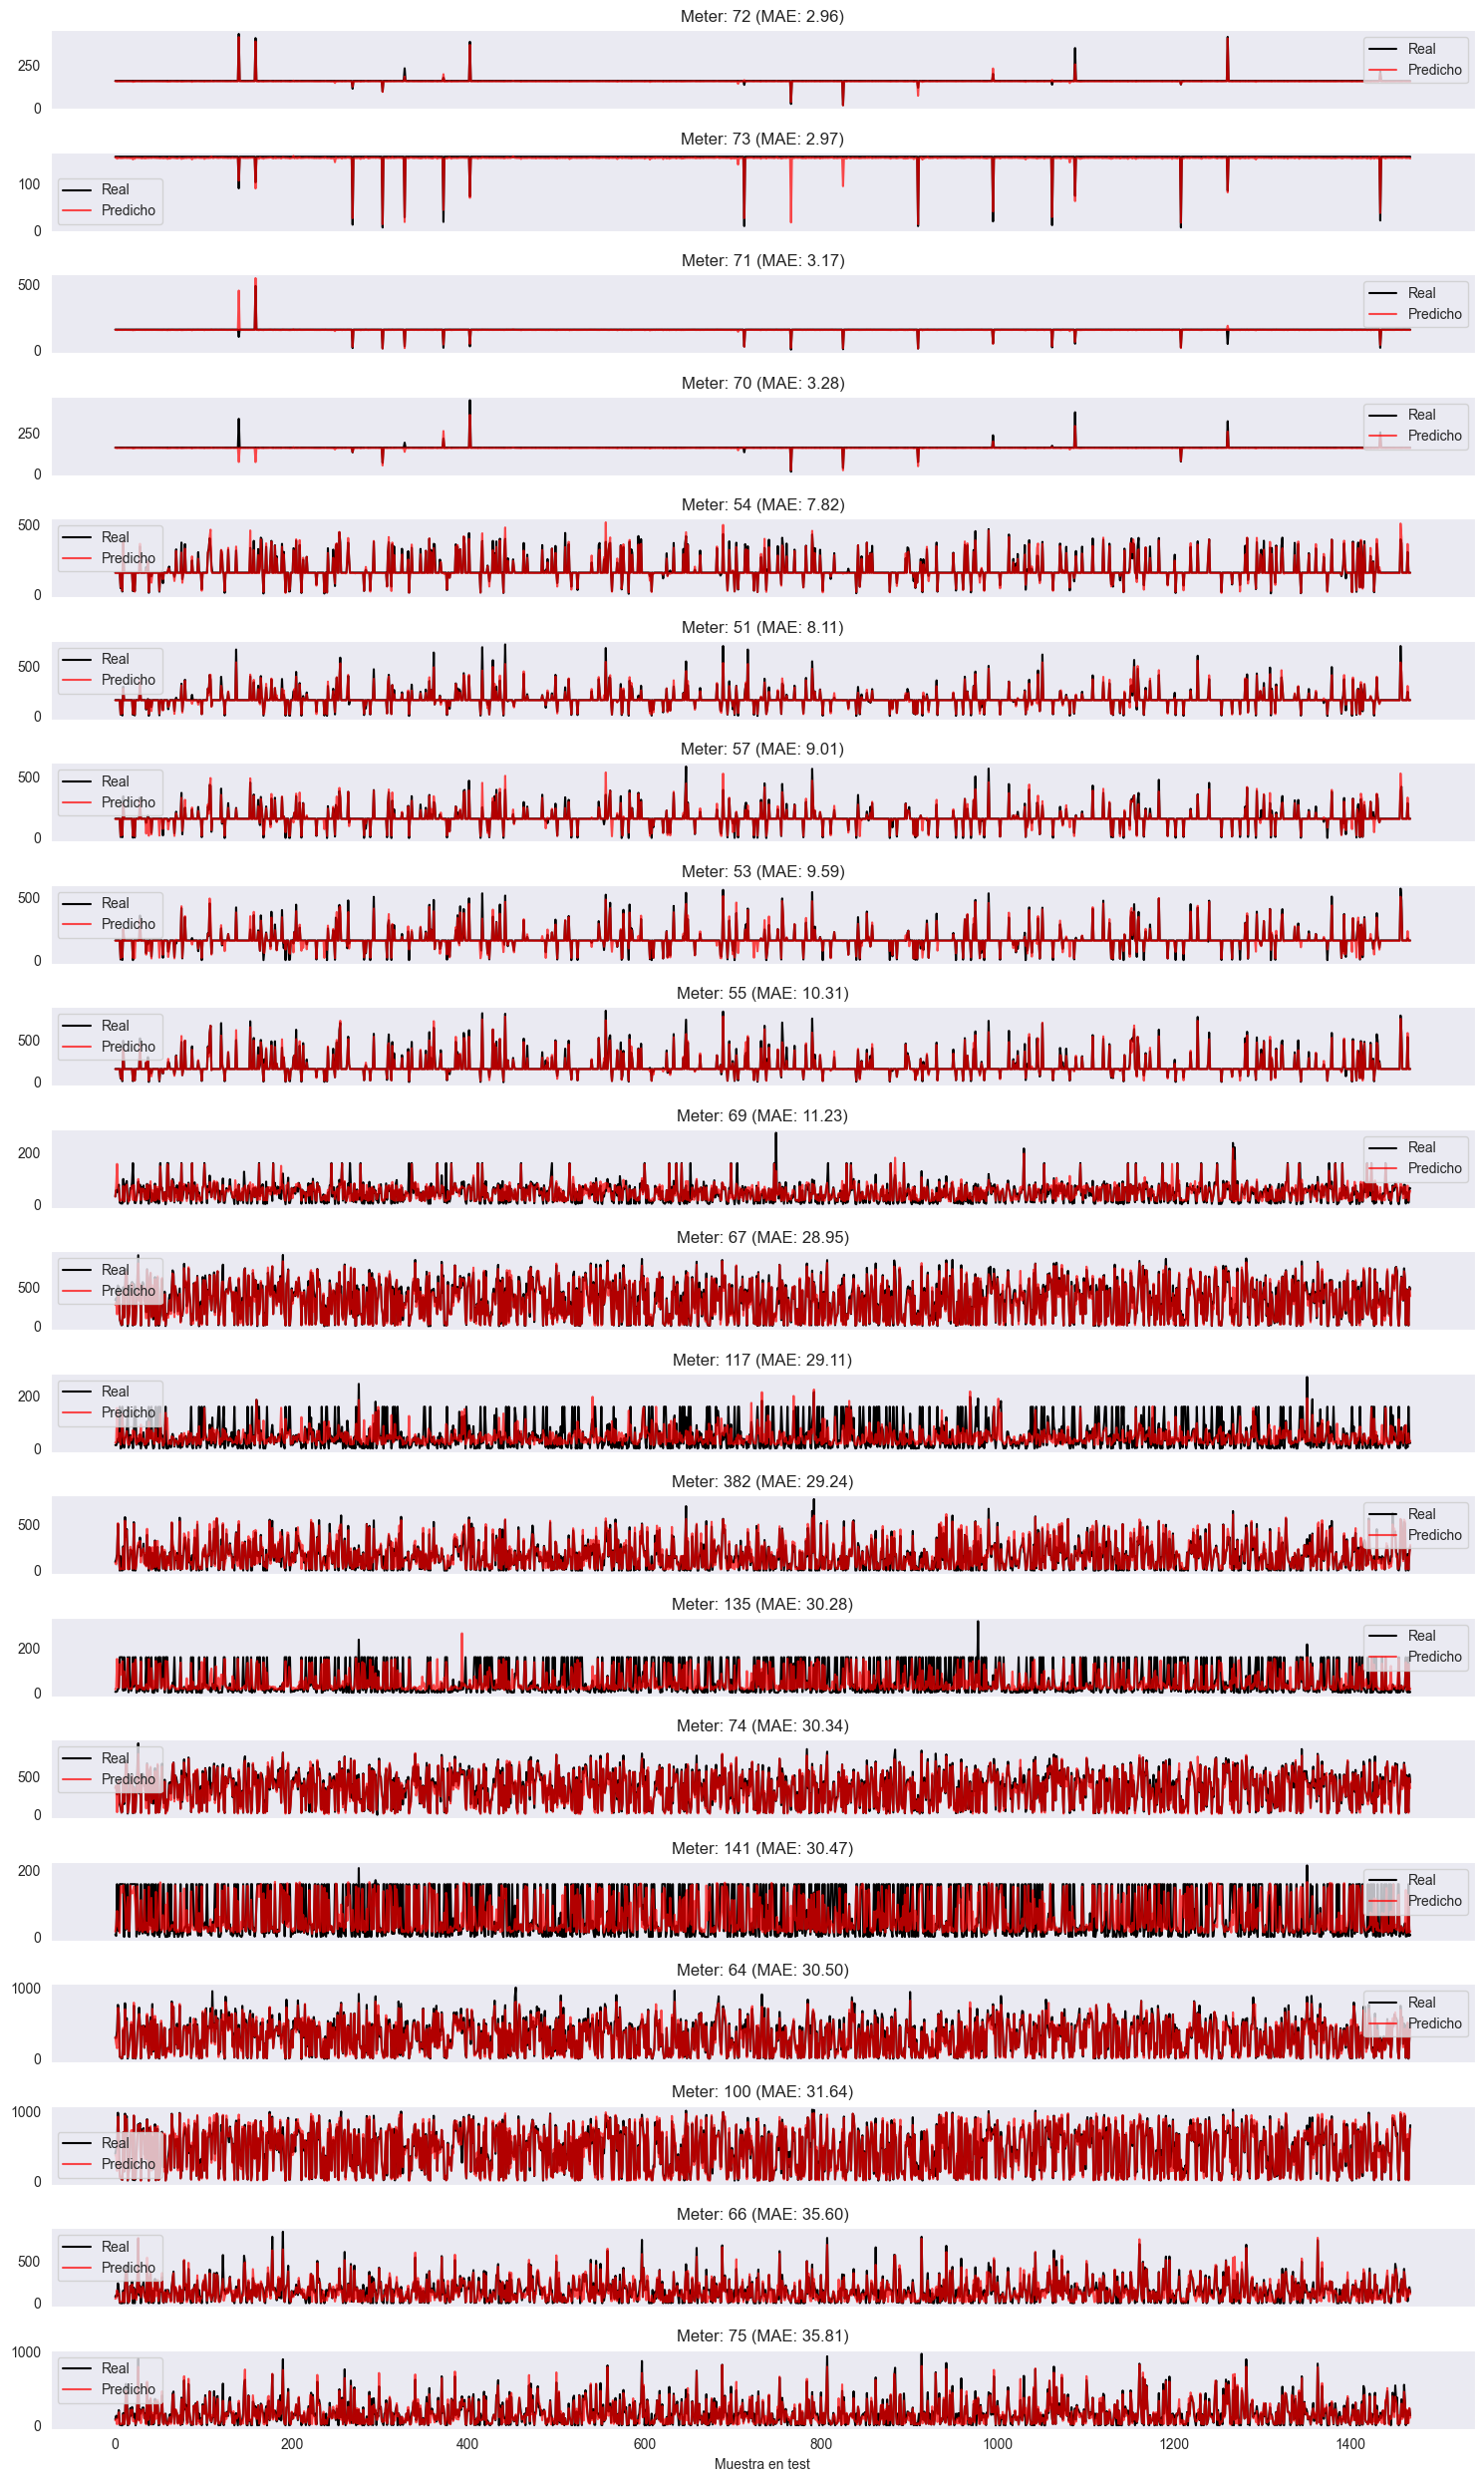
\includegraphics[width=0.75\linewidth]{includes/cap5/graphs/advanced/sid1_10best_10worst_meter_time_series.png}
	\caption{Serie temporal comparativa (predicción vs. real) para los 10 mejores y 10 peores sensores del SourceId 1.}
	\label{fig:sid1_timeseries_best_worst}
\end{figure}

\begin{figure}[H]
	\centering
	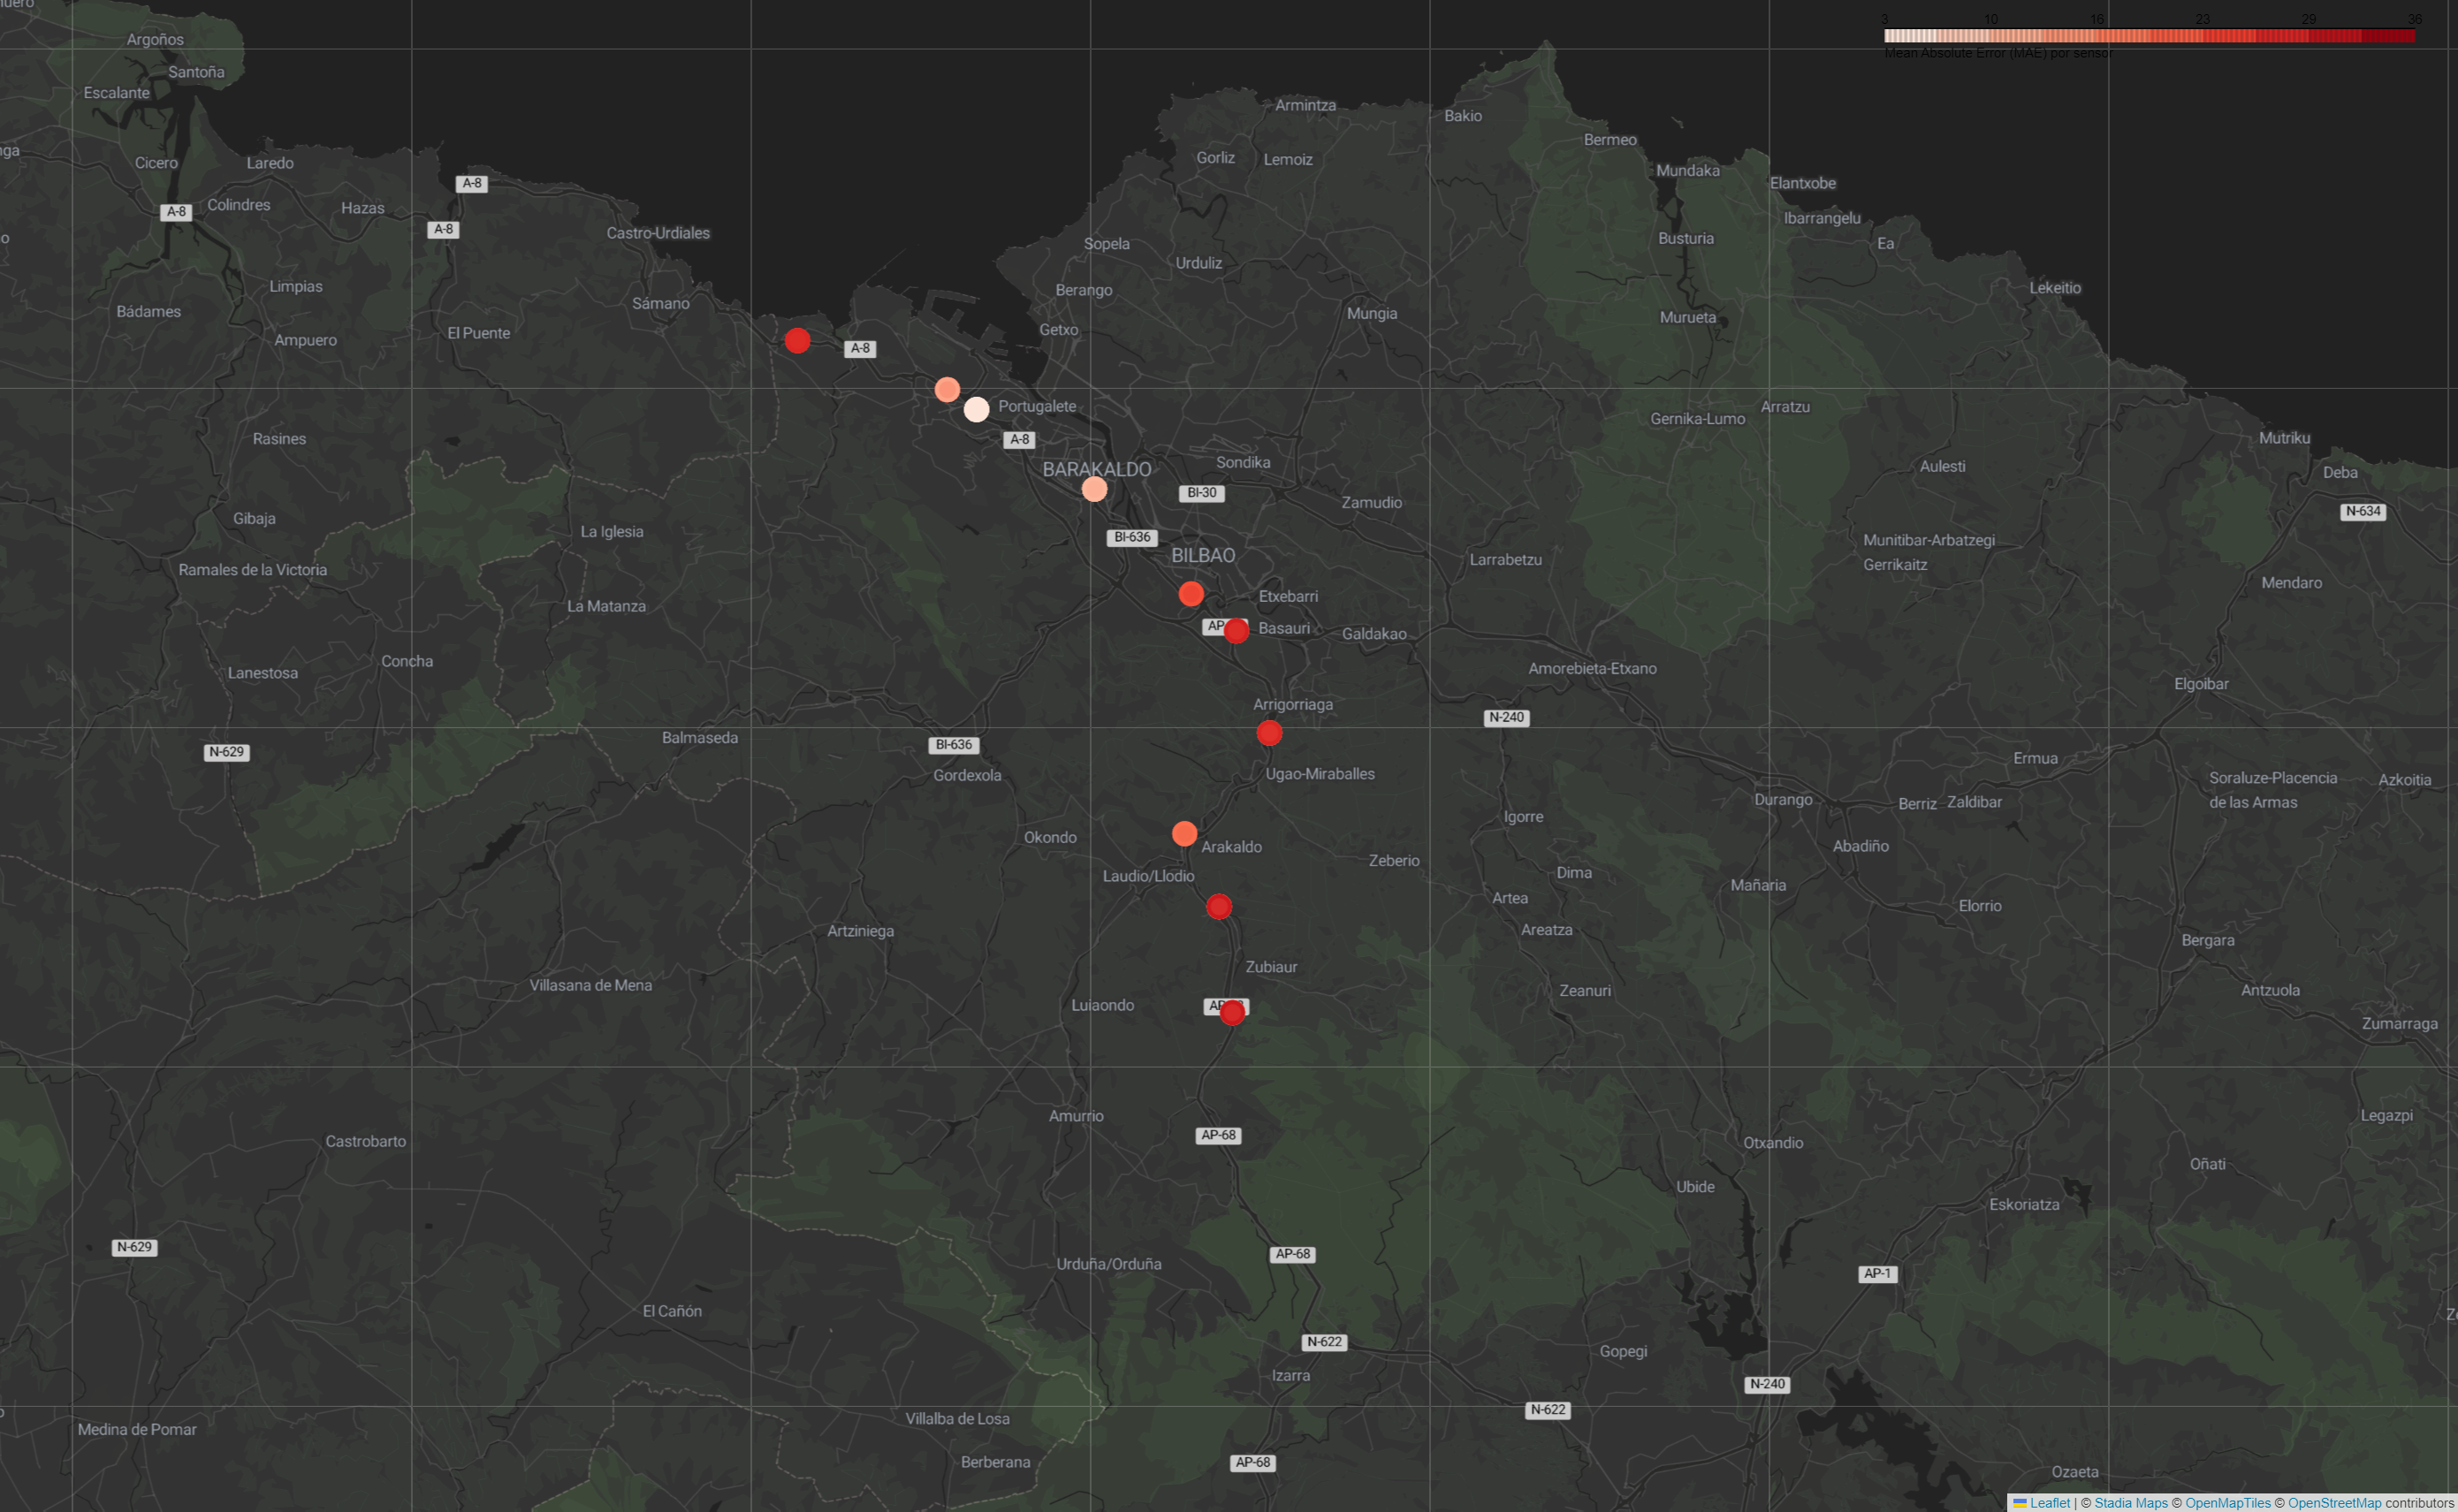
\includegraphics[width=0.9\linewidth]{includes/cap5/graphs/advanced/sid1_meters_error_rate_map.png}
	\caption{Mapa espacial de errores (MAE) para sensores del SourceId 1.}
	\label{fig:sid1_error_map}
\end{figure}

\subsection*{SourceId 2}

\begin{figure}[H]
	\centering
	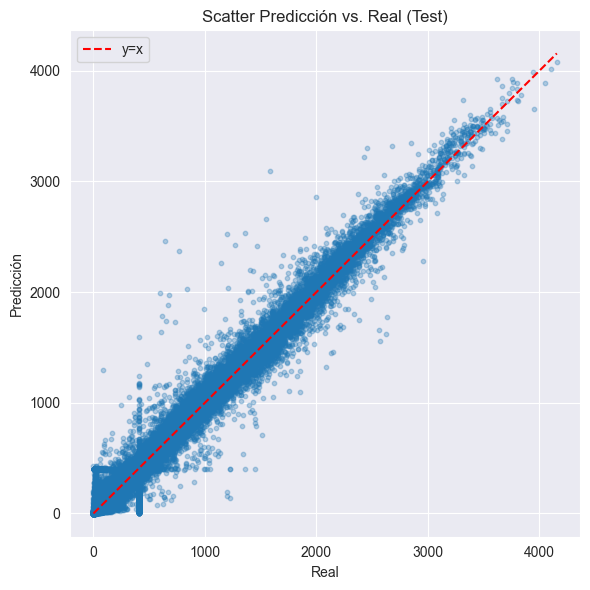
\includegraphics[width=0.75\linewidth]{includes/cap5/graphs/advanced/sid2_scatter_predicted_vs_actual.png}
	\caption{Gráfico de dispersión (predicción vs. valores reales) para SourceId 2.}
	\label{fig:sid2_scatter}
\end{figure}

\begin{figure}[H]
	\centering
	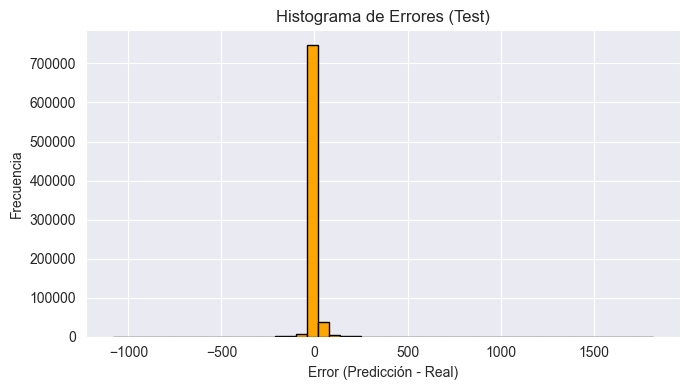
\includegraphics[width=0.75\linewidth]{includes/cap5/graphs/advanced/sid2_error_histogram_predicted_vs_actual.png}
	\caption{Histograma del error absoluto (residual) para SourceId 2.}
	\label{fig:sid2_histograma_error}
\end{figure}

\begin{figure}[H]
	\centering
	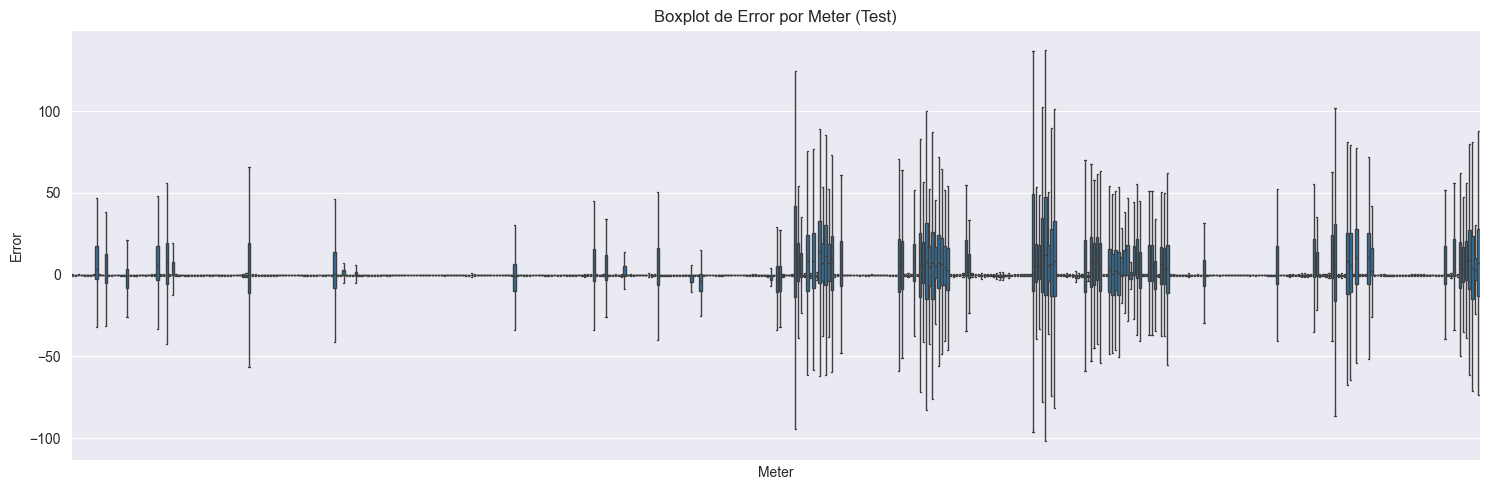
\includegraphics[width=0.75\linewidth]{includes/cap5/graphs/advanced/sid2_all_meters_error_boxplot.png}
	\caption{Boxplot del error absoluto por sensor para todos los sensores del SourceId 2.}
	\label{fig:sid2_boxplot_all}
\end{figure}

\begin{figure}[H]
	\centering
	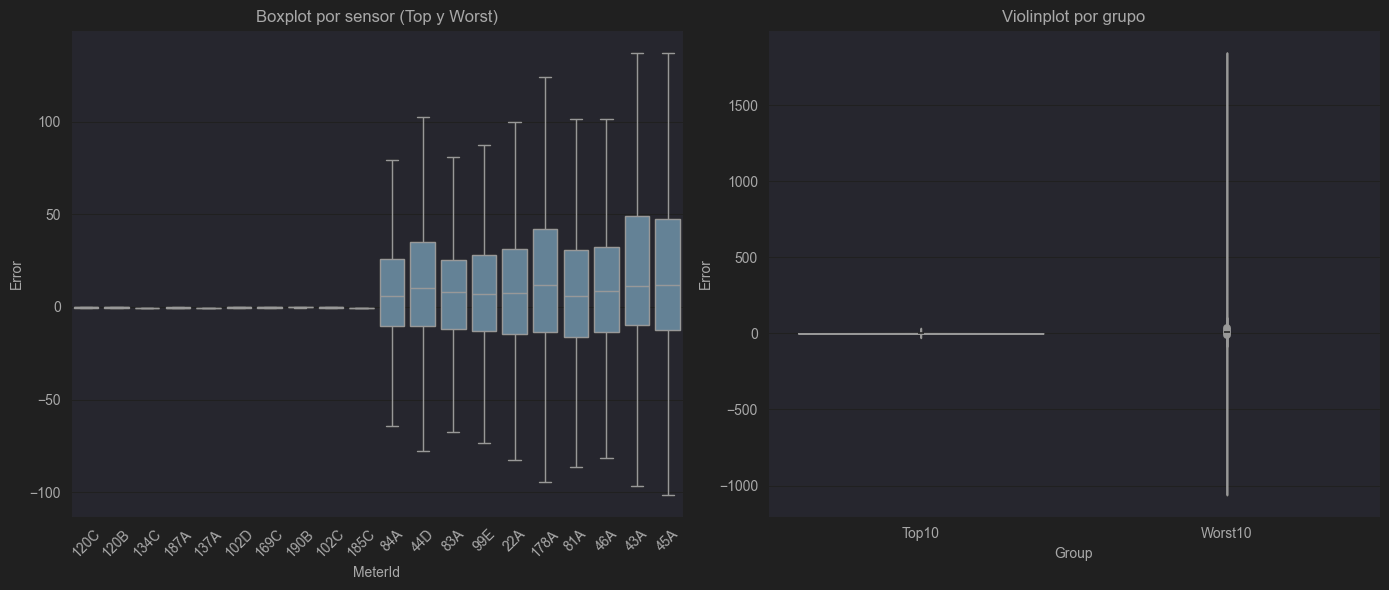
\includegraphics[width=0.75\linewidth]{includes/cap5/graphs/advanced/sid2_10best_10worst_meter_boxplot_violinplot.png}
	\caption{Boxplot y Violinplot de errores para los 10 mejores y los 10 peores sensores del SourceId 2.}
	\label{fig:sid2_violinplot_best_worst}
\end{figure}

\begin{figure}[H]
	\centering
	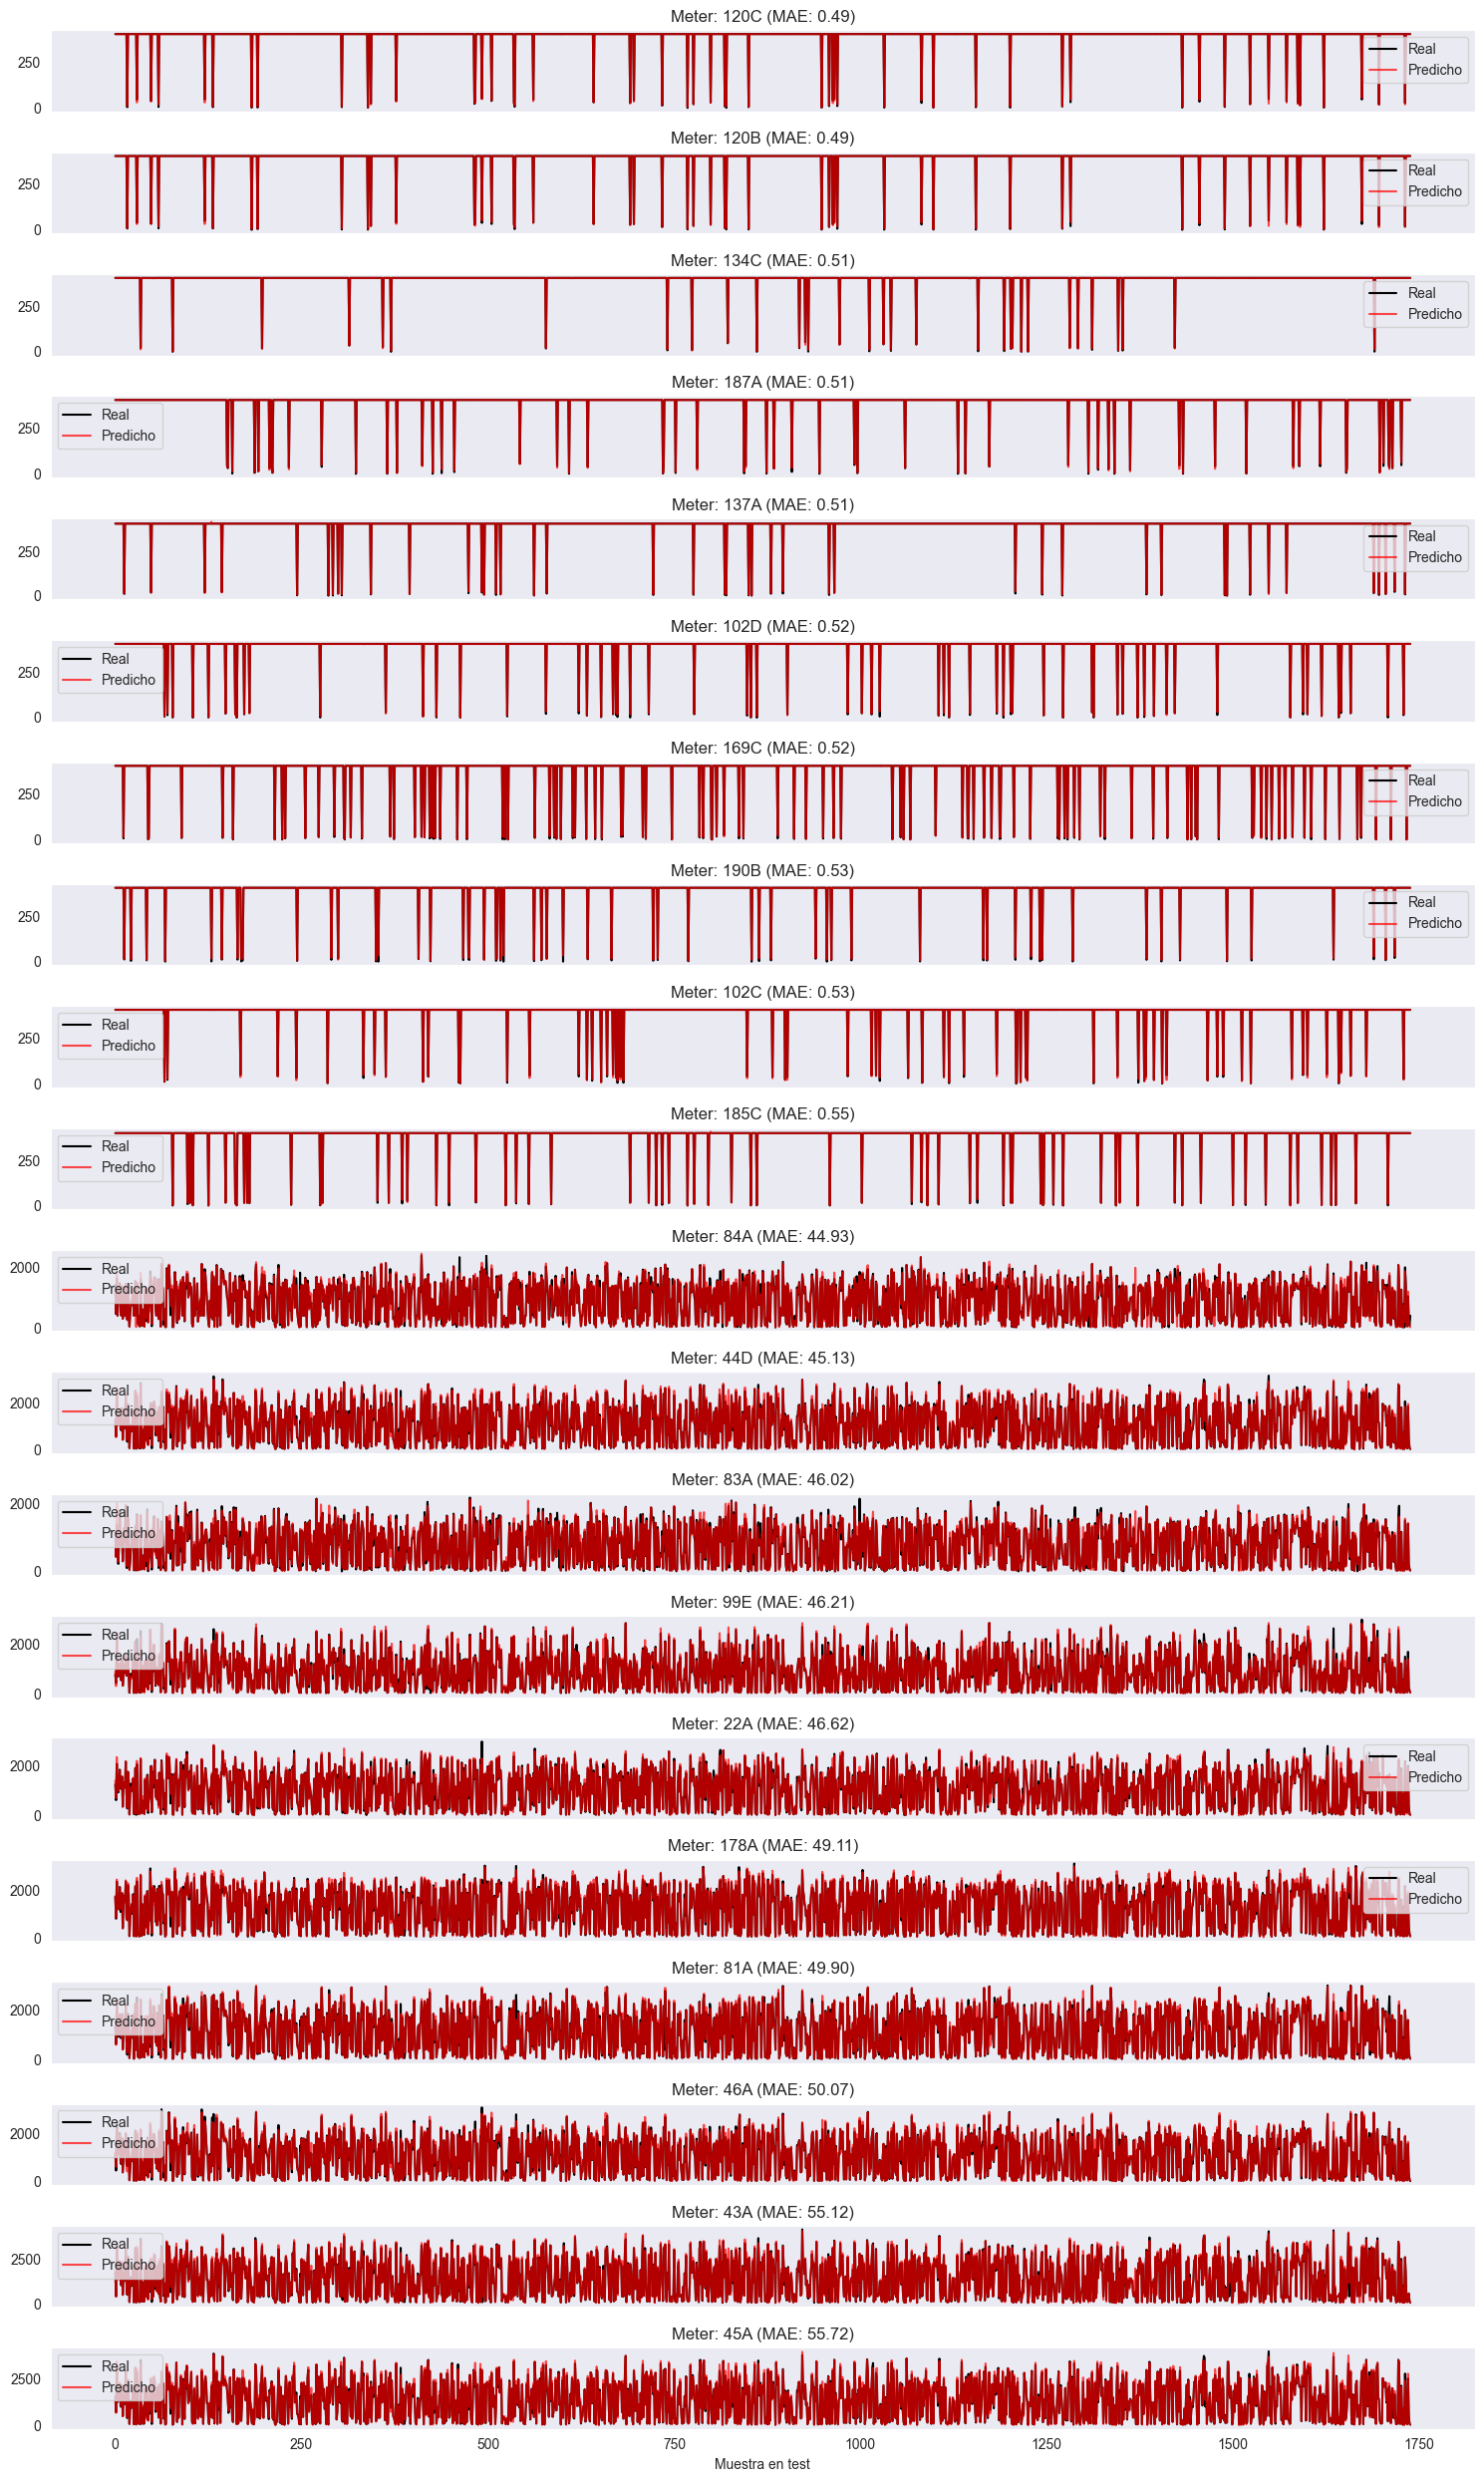
\includegraphics[width=0.75\linewidth]{includes/cap5/graphs/advanced/sid2_10best_10worst_meter_time_series.png}
	\caption{Serie temporal comparativa (predicción vs. real) para los 10 mejores y 10 peores sensores del SourceId 2.}
	\label{fig:sid2_timeseries_best_worst}
\end{figure}

\begin{figure}[H]
	\centering
	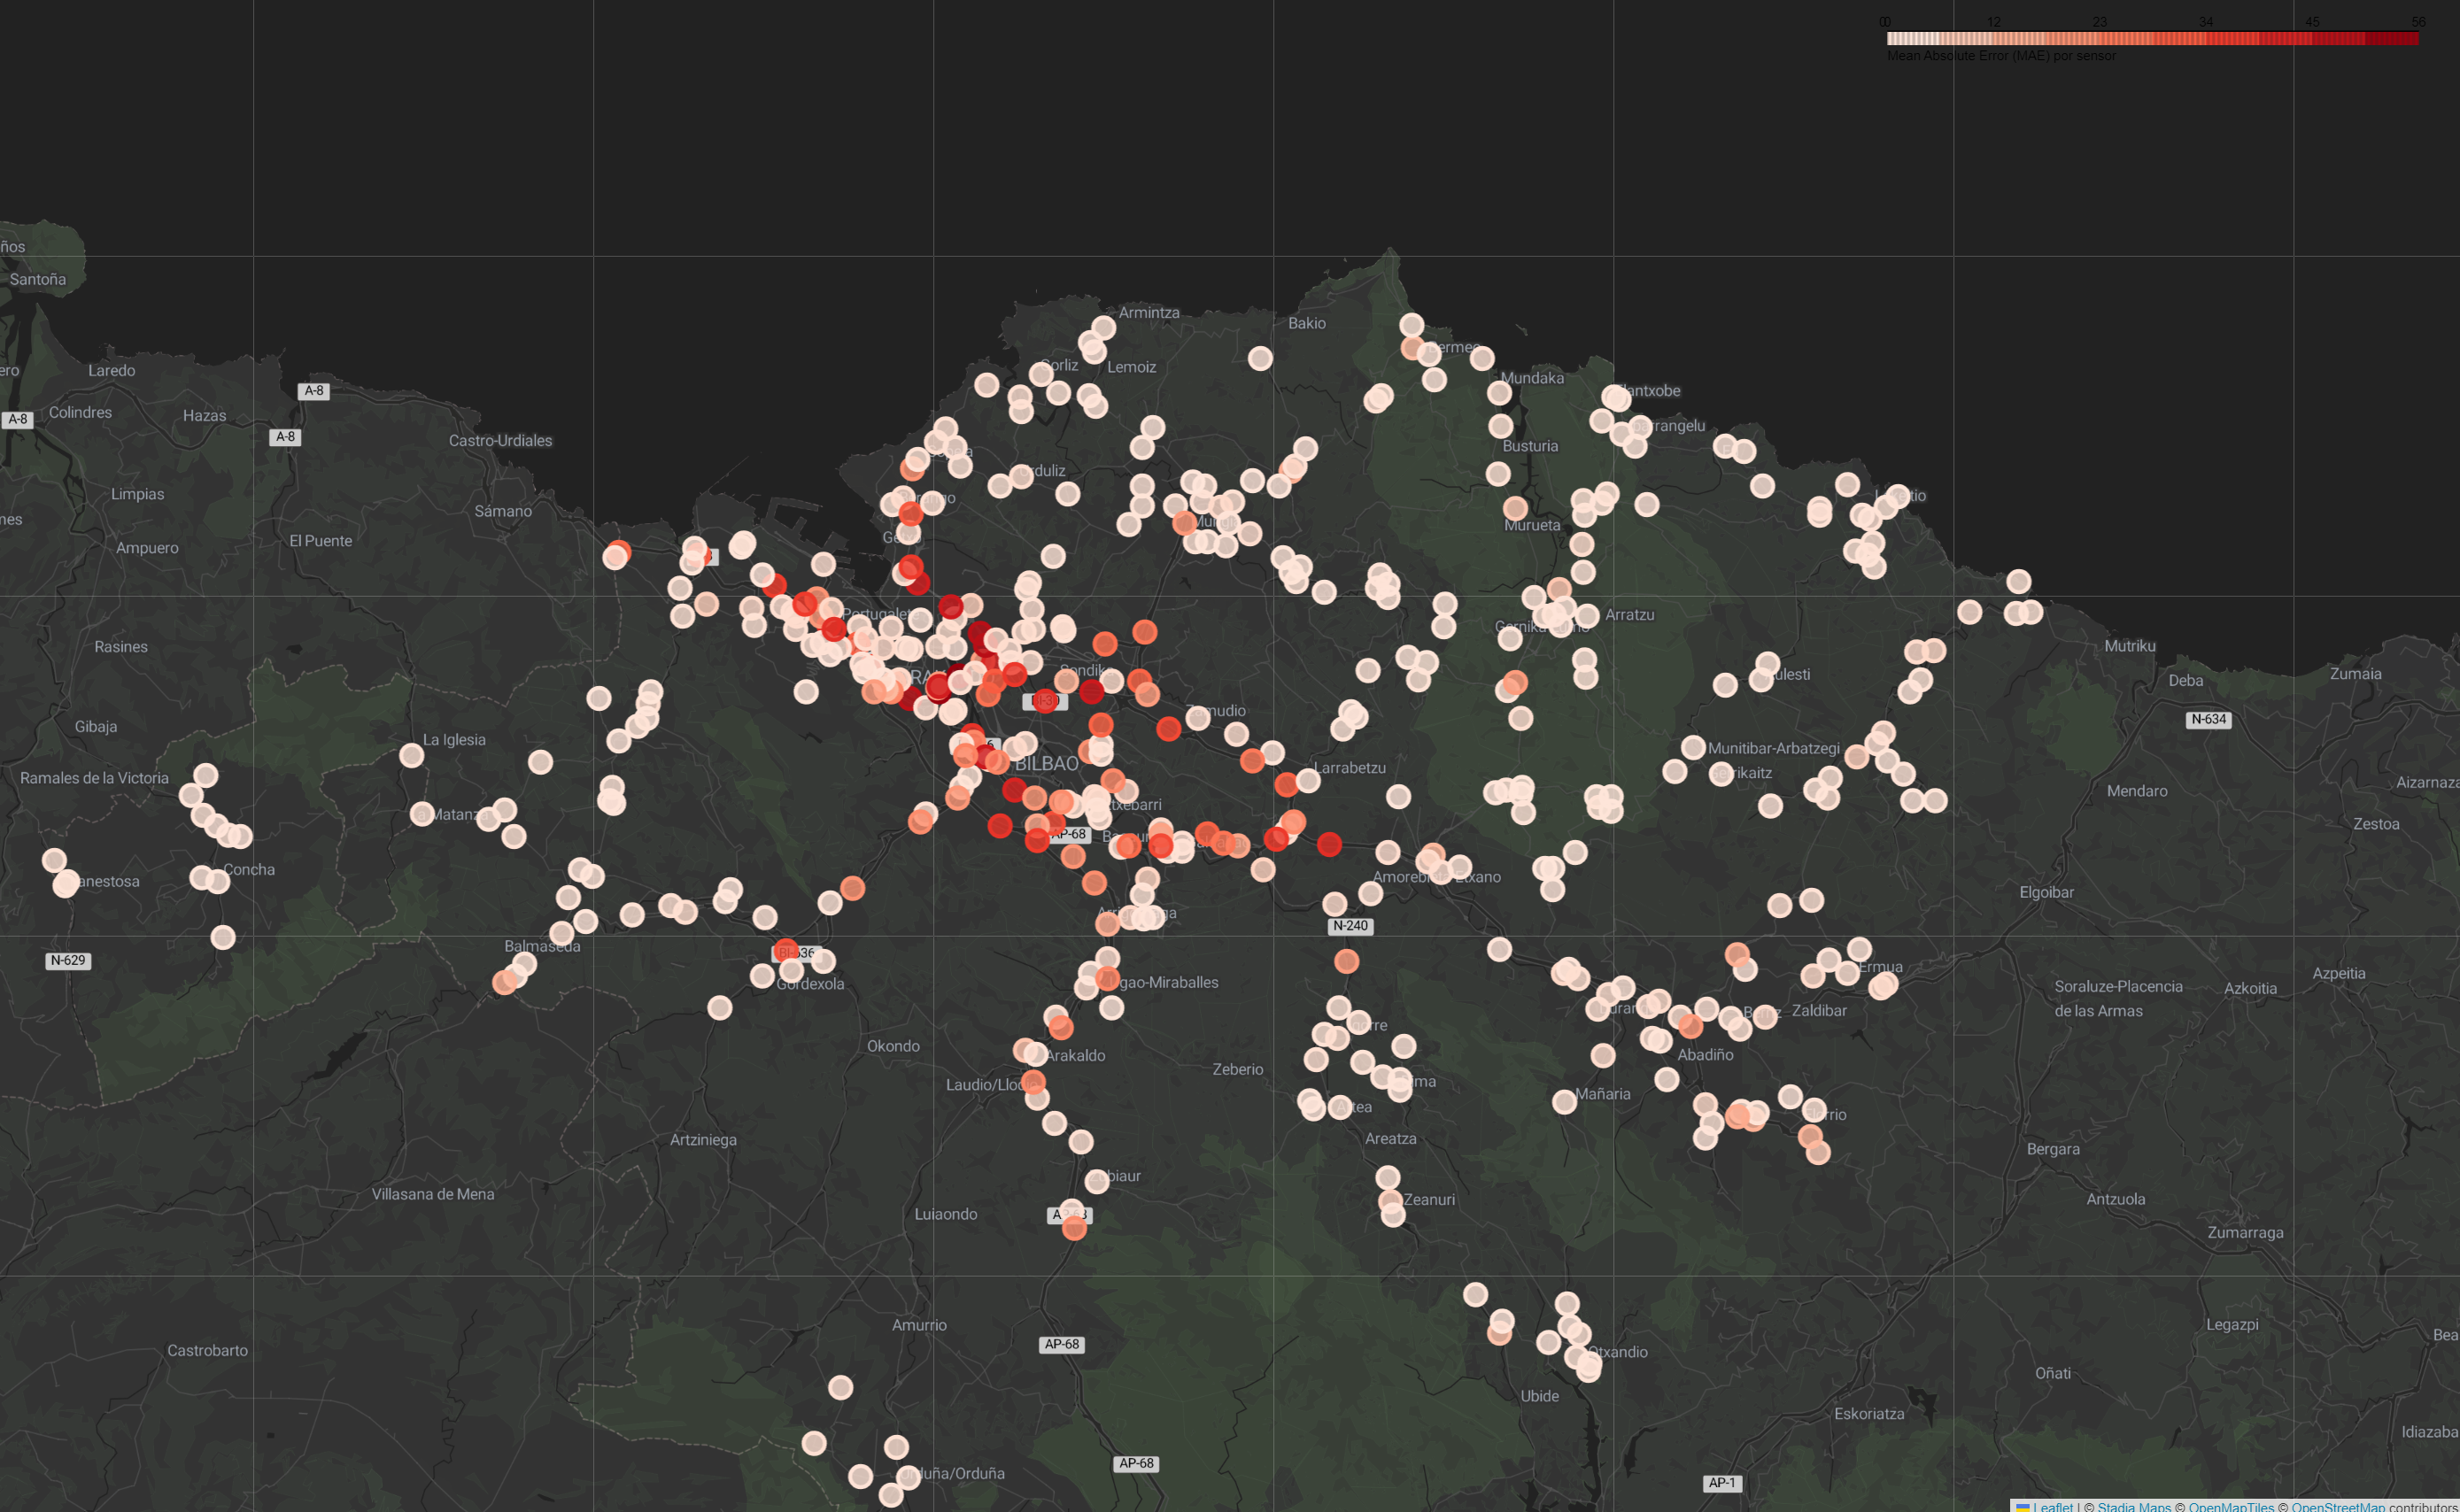
\includegraphics[width=0.9\linewidth]{includes/cap5/graphs/advanced/sid2_meters_error_rate_map.png}
	\caption{Mapa espacial de errores (MAE) para sensores del SourceId 2.}
	\label{fig:sid2_error_map}
\end{figure}

\subsection*{SourceId 5}

\begin{figure}[H]
	\centering
	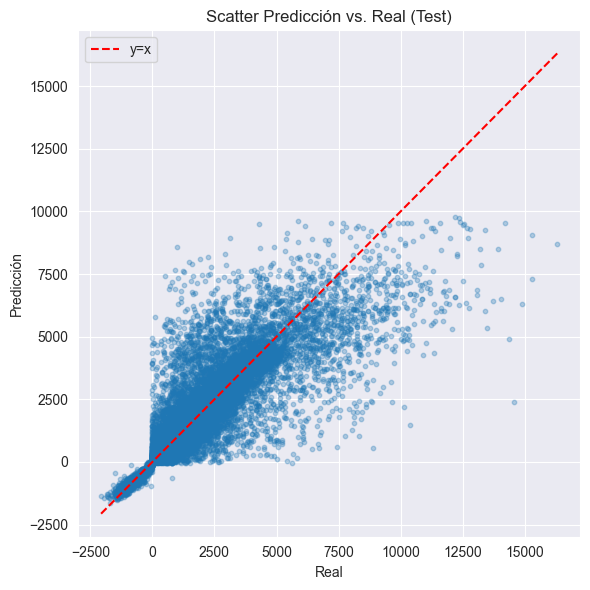
\includegraphics[width=0.75\linewidth]{includes/cap5/graphs/advanced/sid5_scatter_predicted_vs_actual.png}
	\caption{Gráfico de dispersión (predicción vs. valores reales) para SourceId 5.}
	\label{fig:sid5_scatter}
\end{figure}

\begin{figure}[H]
	\centering
	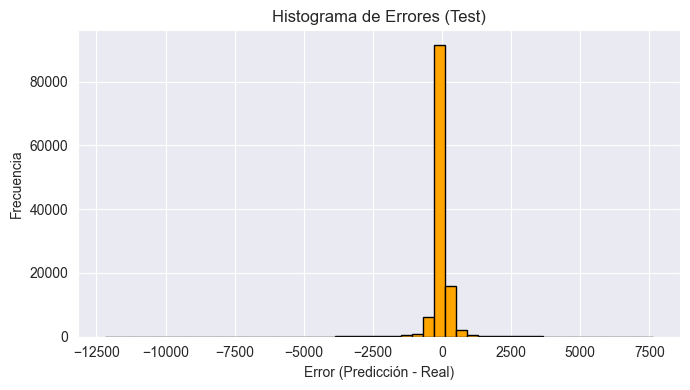
\includegraphics[width=0.75\linewidth]{includes/cap5/graphs/advanced/sid5_error_histogram_predicted_vs_actual.png}
	\caption{Histograma del error absoluto (residual) para SourceId 5.}
	\label{fig:sid5_histograma_error}
\end{figure}

\begin{figure}[H]
	\centering
	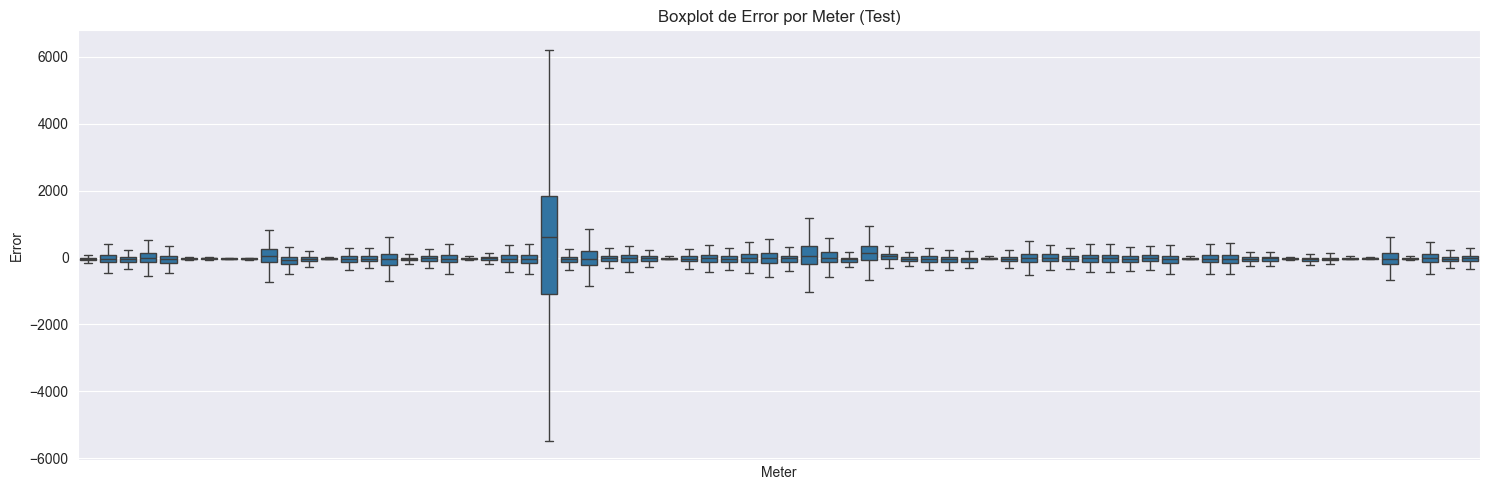
\includegraphics[width=0.75\linewidth]{includes/cap5/graphs/advanced/sid5_all_meters_error_boxplot.png}
	\caption{Boxplot del error absoluto por sensor para todos los sensores del SourceId 5.}
	\label{fig:sid5_boxplot_all}
\end{figure}

\begin{figure}[H]
	\centering
	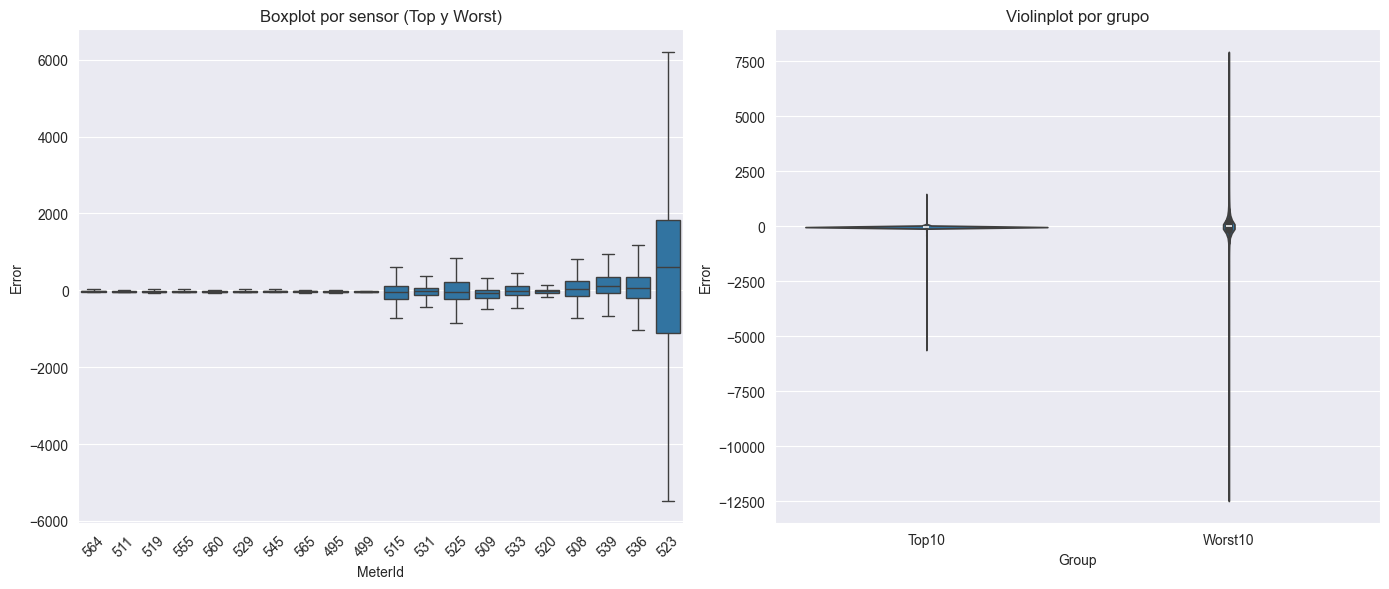
\includegraphics[width=0.75\linewidth]{includes/cap5/graphs/advanced/sid5_10best_10worst_meter_boxplot_violinplot.png}
	\caption{Boxplot y Violinplot de errores para los 10 mejores y los 10 peores sensores del SourceId 5.}
	\label{fig:sid5_violinplot_best_worst}
\end{figure}

\begin{figure}[H]
	\centering
	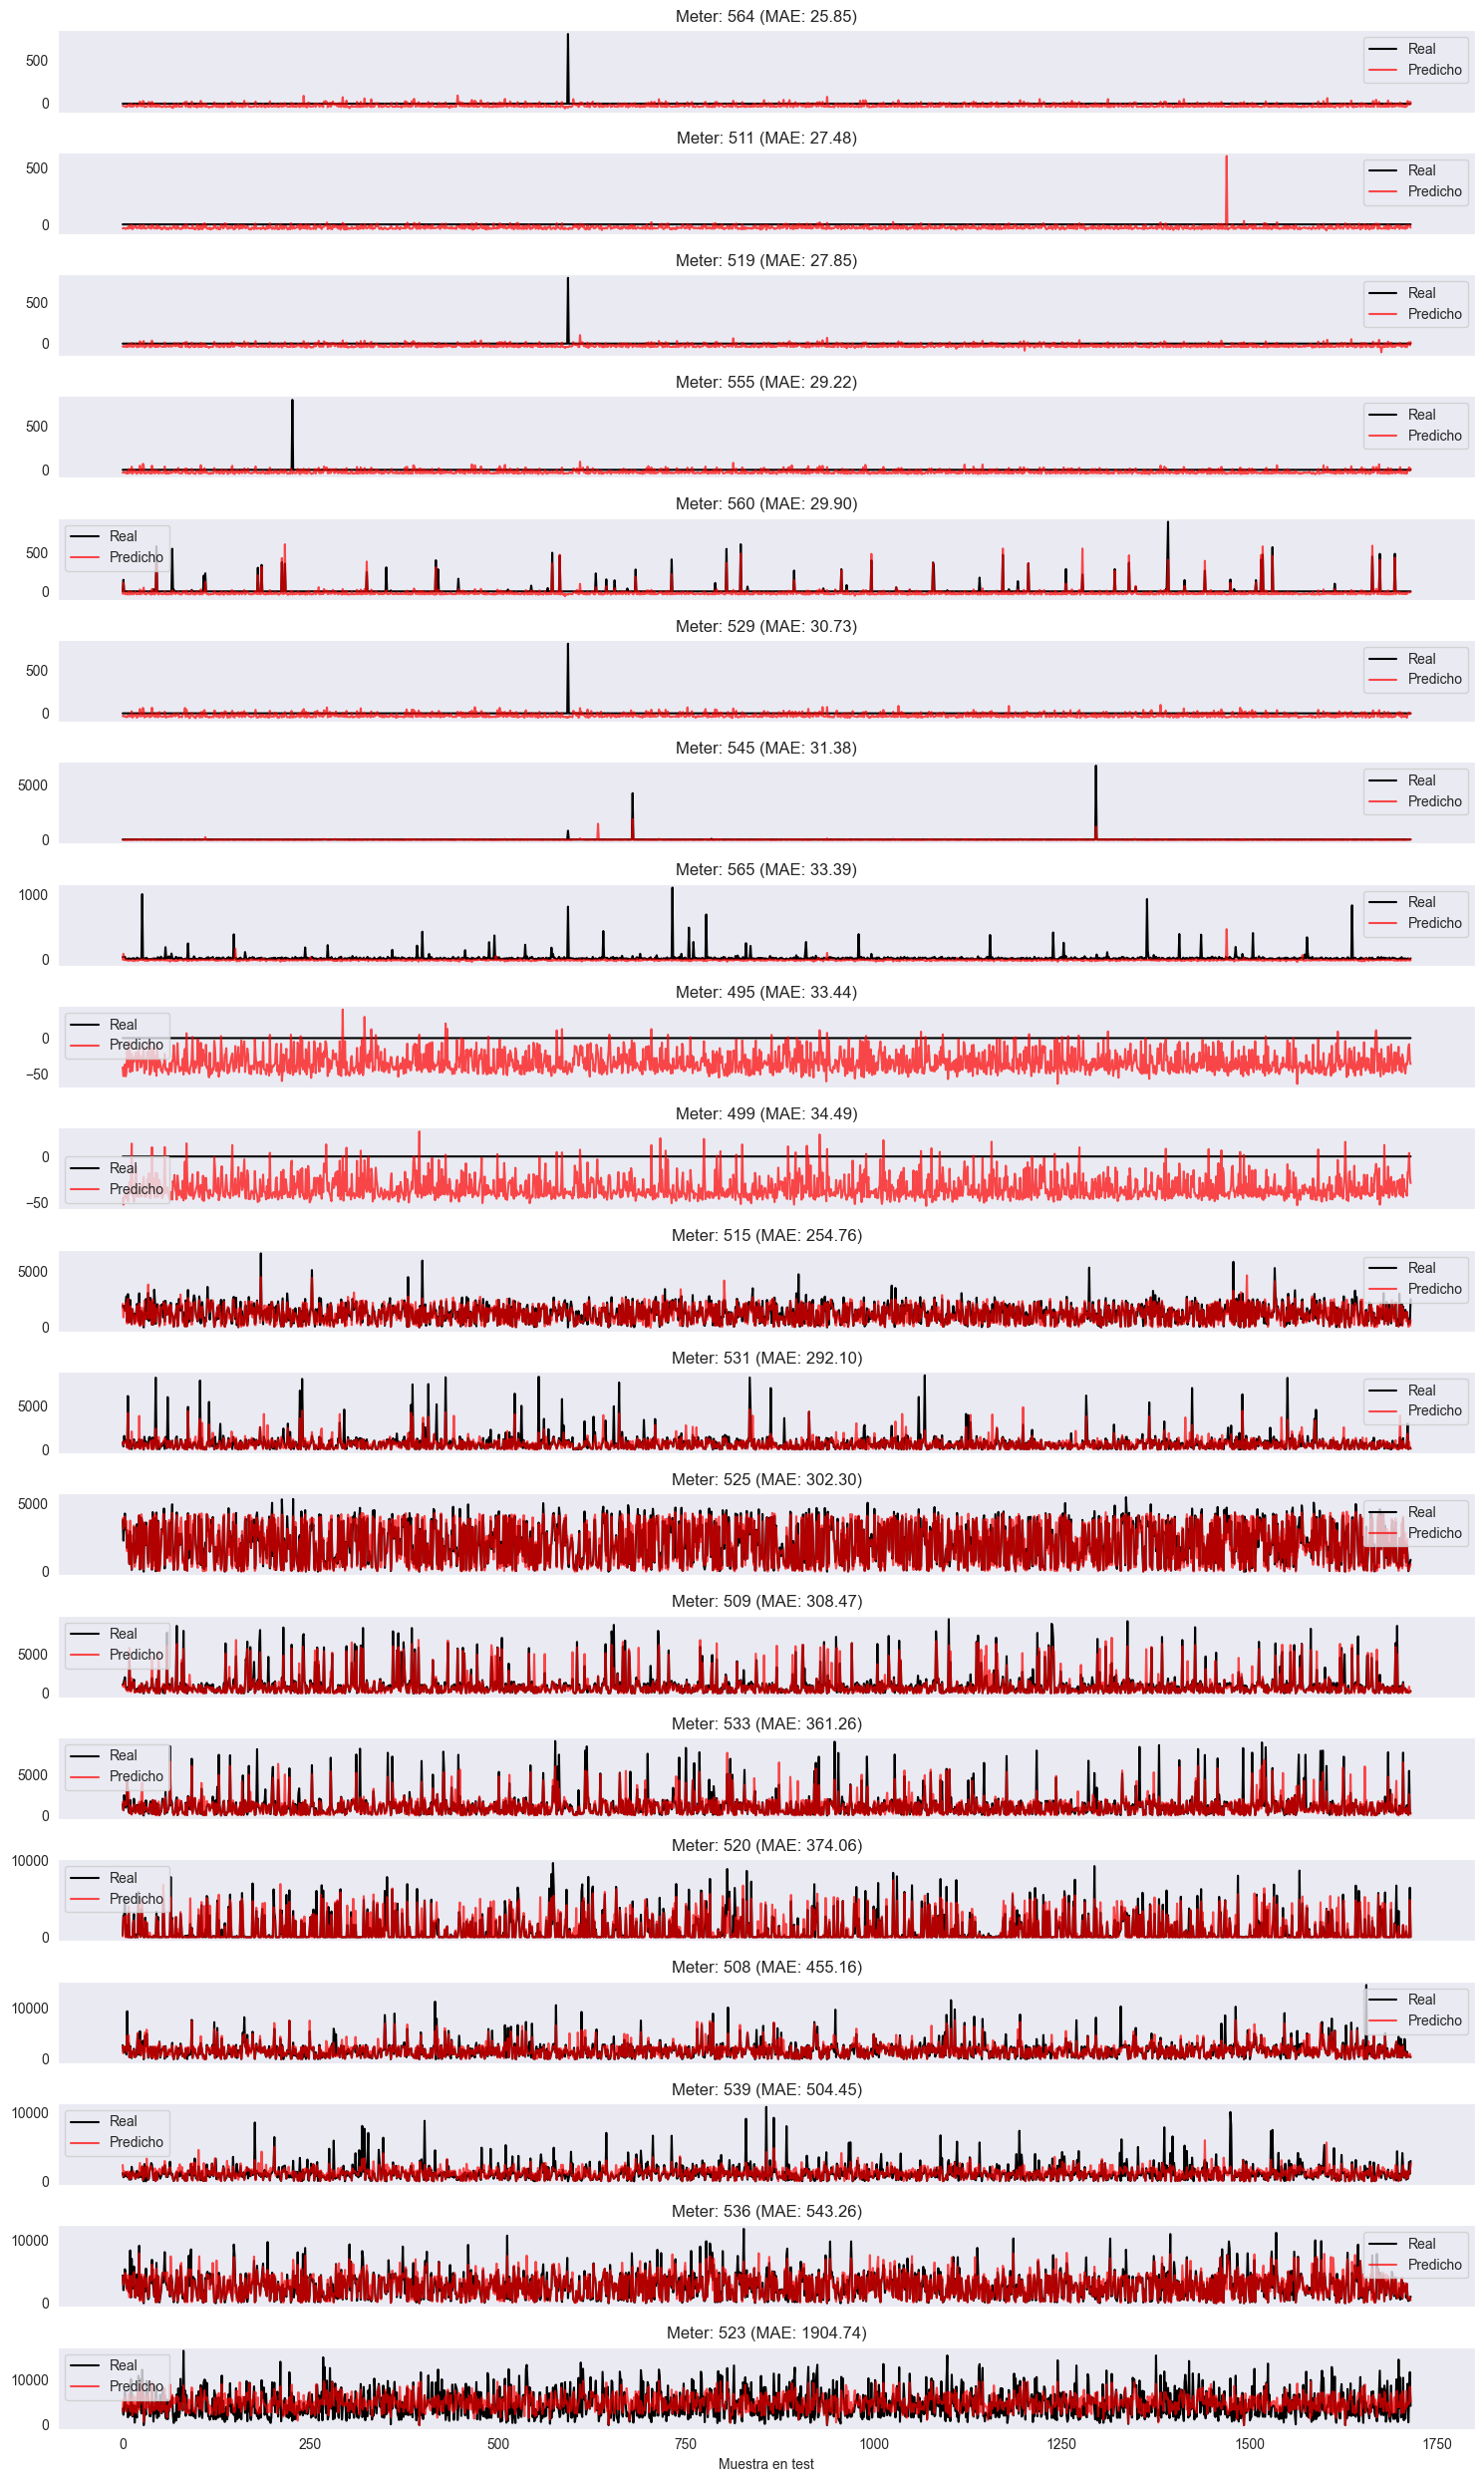
\includegraphics[width=0.75\linewidth]{includes/cap5/graphs/advanced/sid5_10best_10worst_meter_time_series.png}
	\caption{Serie temporal comparativa (predicción vs. real) para los 10 mejores y 10 peores sensores del SourceId 5.}
	\label{fig:sid5_timeseries_best_worst}
\end{figure}

\begin{figure}[H]
	\centering
	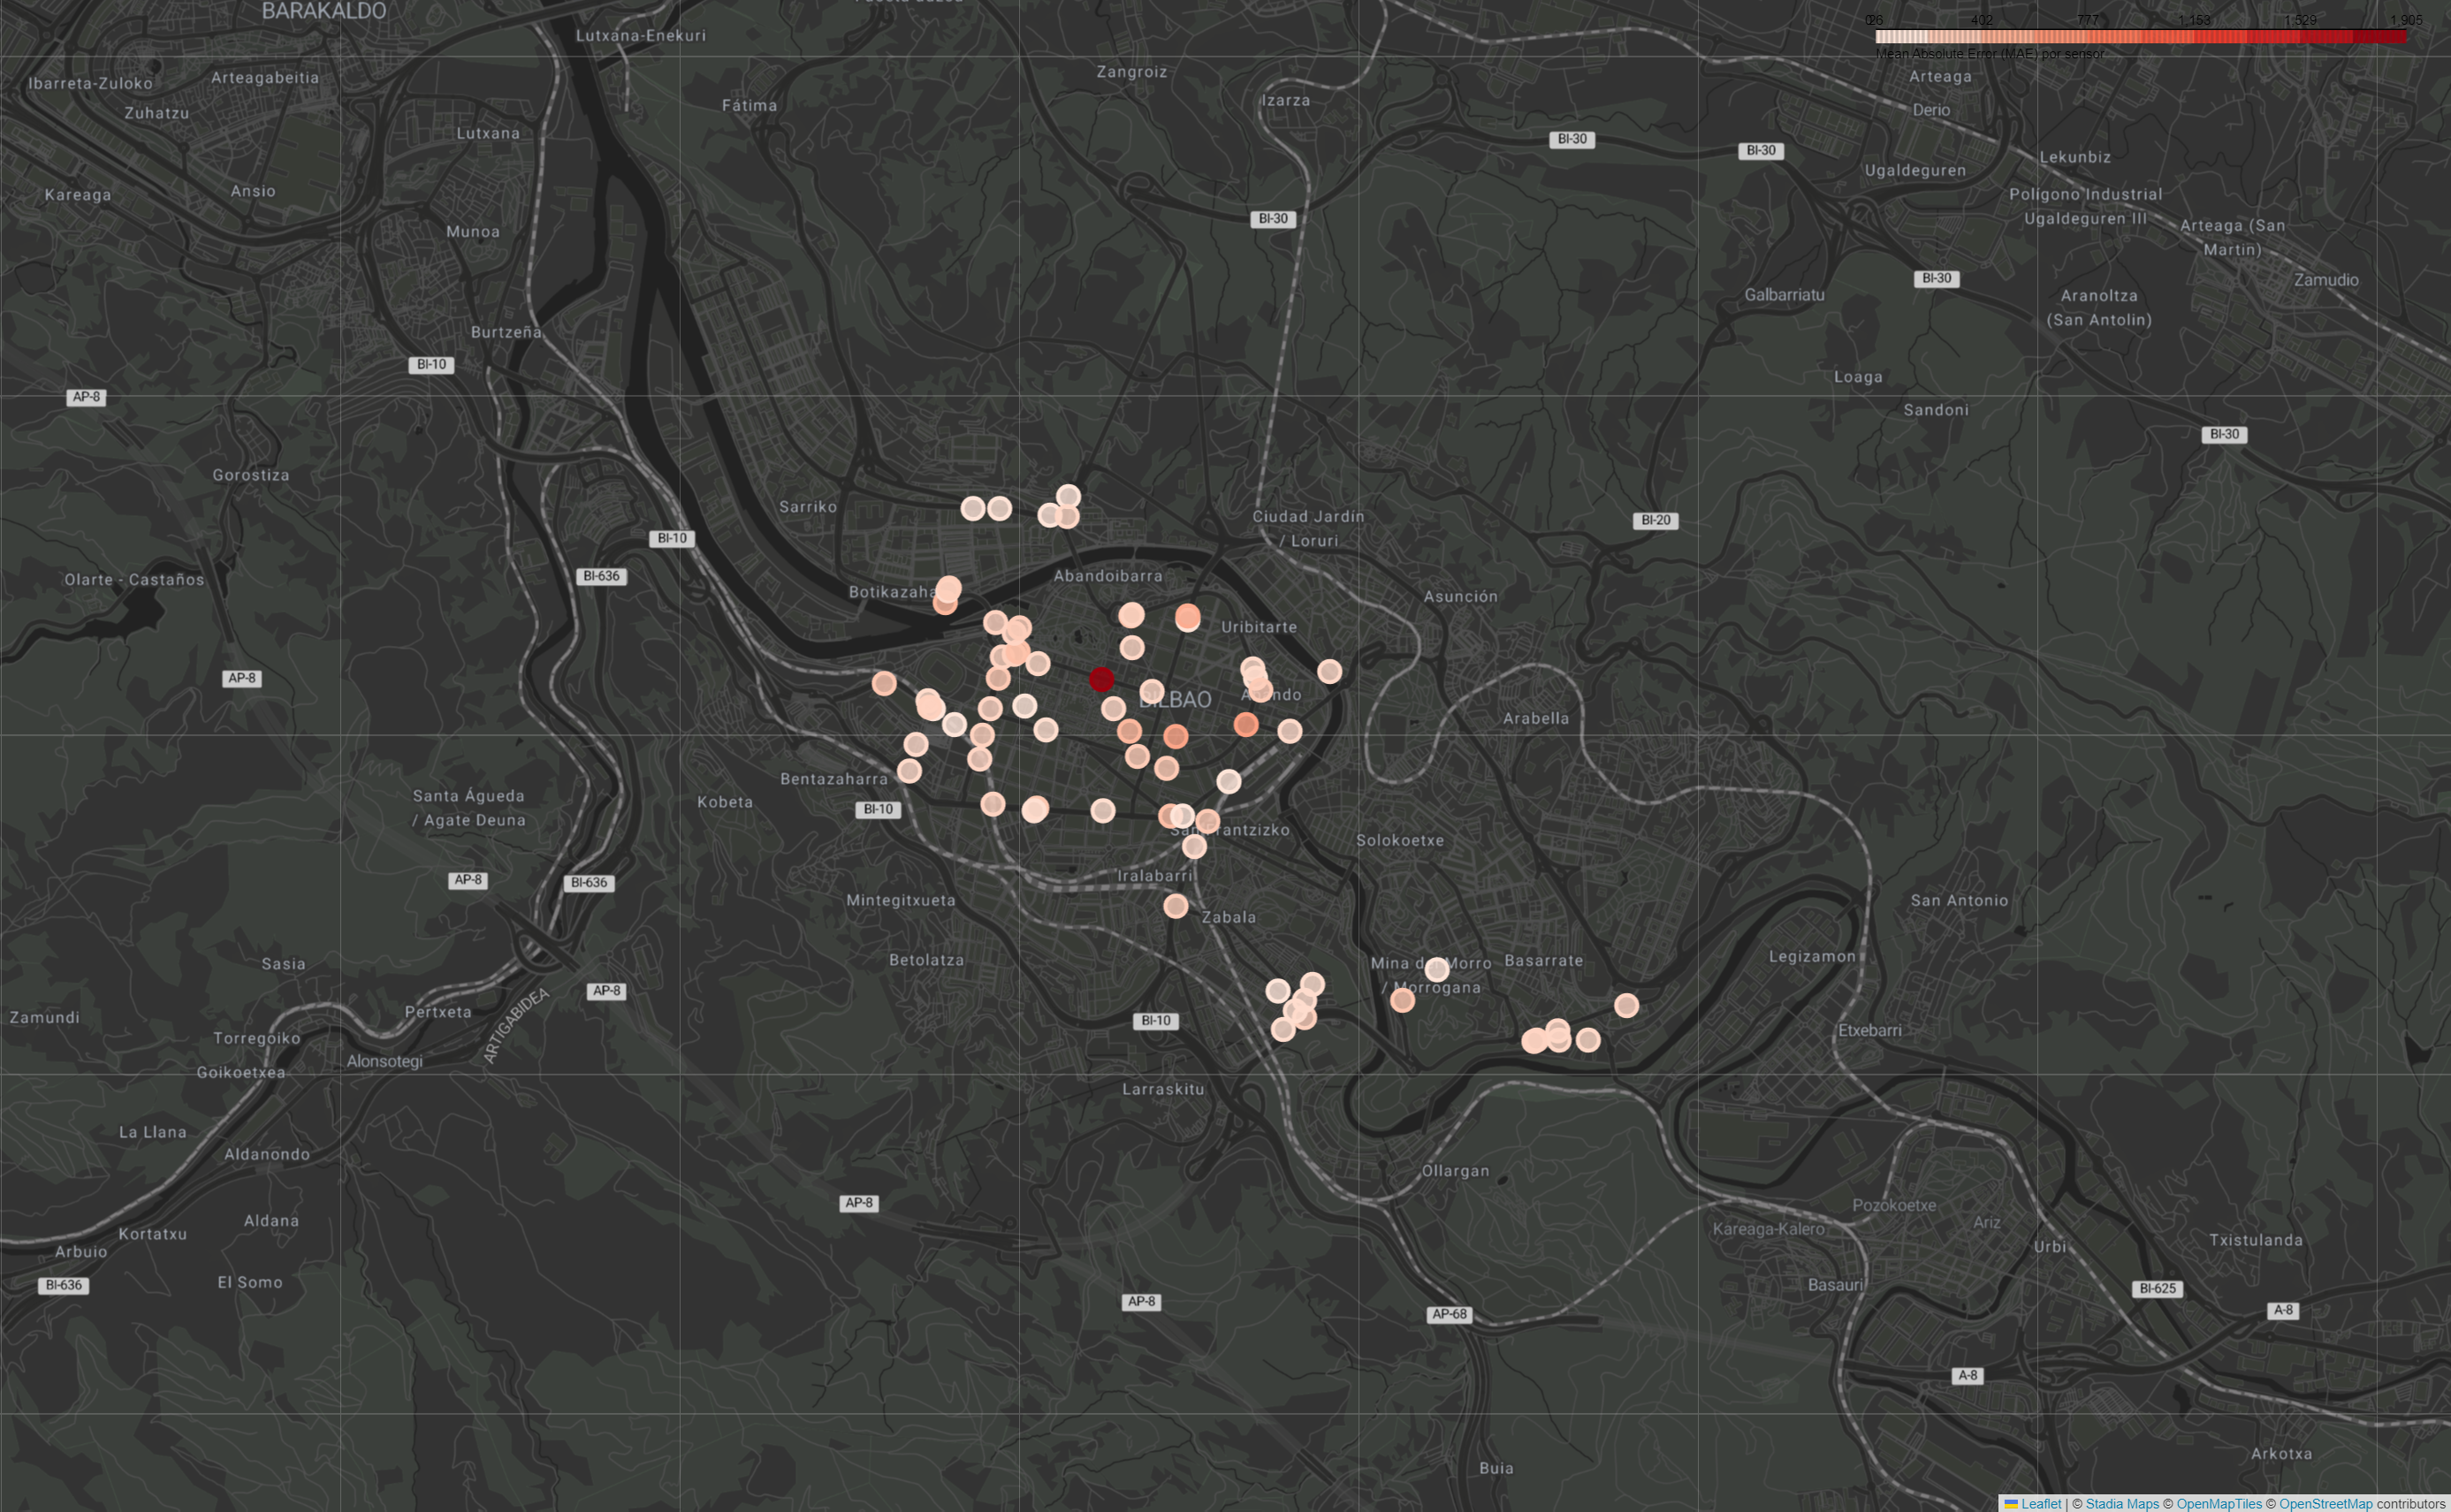
\includegraphics[width=0.9\linewidth]{includes/cap5/graphs/advanced/sid5_meters_error_rate_map.png}
	\caption{Mapa espacial de errores (MAE) para sensores del SourceId 5.}
	\label{fig:sid5_error_map}
\end{figure}


